\chapter{Methodology}

This chapter introduces notations as well as the mathematical models and software tools used in this thesis. It starts with describing the data generation pipeline that is used to generate synthetic data. Subsequently, the Object-Detection network is explained. Finally, two datasets used for evaluation are introduced.

\section{Data Generation Pipeline}
\label{sec:datagen:method}
\begin{figure}[htbp]
	\centering
	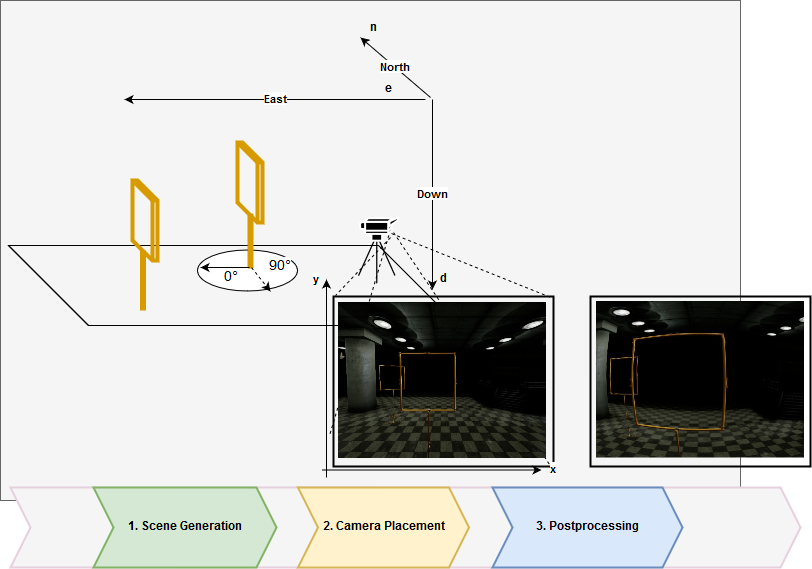
\includegraphics[width=0.9\textwidth]{fig/datagen_notation}
	\caption{Notation and data generation process. In the first step a scene is created which defines the environment and background. The second step places the camera in the environment and creates a 2D view of the scene. The third step applies further image transformations. The coordinate system in 3D is \ac{NED} originating at the initial position of the camera. In 2D, positions are defined in Cartesian coordinates originating at the bottom left. With a rotation of 0° the object appears as an empty square, with 90° as a straight line.}
	\label{fig:training:datagen_notation}
\end{figure}

An overview of the data generation pipeline can be seen in \Cref{fig:training:datagen_notation}. In the first step a scene is created in which the objects of interest as well as the camera are placed. In 3D space position and orientation (pose) of each object are determined by its translation $\textbf{t} = [x,y,z]$ and rotation $\textbf{r}={\phi, \theta, \psi}$. The used coordinate system is \ac{NED} while the center of origin is placed at the initial position of the camera.

A view projection yields an image through the lens of the camera. The coordinates of each point in 3D space are projected on the 2D image plane. The position of each point in the image space is defined by $\textbf{p} = [p_x,p_y]$. The origin is on the bottom left of the image.\todo{some details about the projection?}

These steps are implemented using \textit{Epic}'s \textit{UnrealEngine}\cite{unreal} and its \textit{AirSim}-Plug-In\cite{airsim} by \textit{Microsoft}. This allows the creation of environments using \ac{CAD} models, as well as the automatic placement of the camera in C++. The tool is extended to store the location of a bounding box that surrounds an object in the environment. This allows the automatic generation of ground truth labels while the camera is placed.

The \textit{UnrealEngine} contains a profound amount of photorealistic image effects. However, their use with data generation tool would require a deep understanding of graphical programming and a substantial amount of work. Hence, the final post processing step is implemented using the image processing library \textit{OpenCV} in Python. This also allows to study the incorporation of particular sensor effects or image augmentation while training the network.

All source code is made publicly available at \url{https://github.com/phildue/datagen.git}.

\subsection{Environments}
\label{sec:environments}
Images can appear substantially different depending on the particular environment in which they are taken. The light conditions in an indoor scene with artificial light are substantially different than the ones outdoors in sunlight. The environment also influences the appearance of an object and therefore its detection.

In order to train and evaluate the detection of \acp{EWFO} in different conditions, three environments are created. A black environment serves as base to replace the background with existing images. Furthermore, three indoor base environments are created that fully simulate illumination and background. An overview can be seen in \Cref{fig:environments}. Within the environment light conditions, background textures, object locations can be changed manually. The environments are described in the following:

\begin{enumerate}
	\item \textit{Dark:} The environment is a room without windows, only containing artificial light sources. 
	\item \textit{Daylight:} The environment is a room with windows along all walls that allow daylight to illuminate the room. The windows can lead to strong variations in the contrast between different parts of the object.
	\item \textit{IROS:} The environment resembles the room of the \ac{IROS} Autonomous Drone Race 2018. The light sources stem from a window front at one side of the room, as well as artificial light sources at the ceiling. Depending on the view point, the object might appear against bright or dark background.
\end{enumerate}

\begin{figure}[hbtp]
	\centering
	\begin{minipage}{0.3\textwidth}
		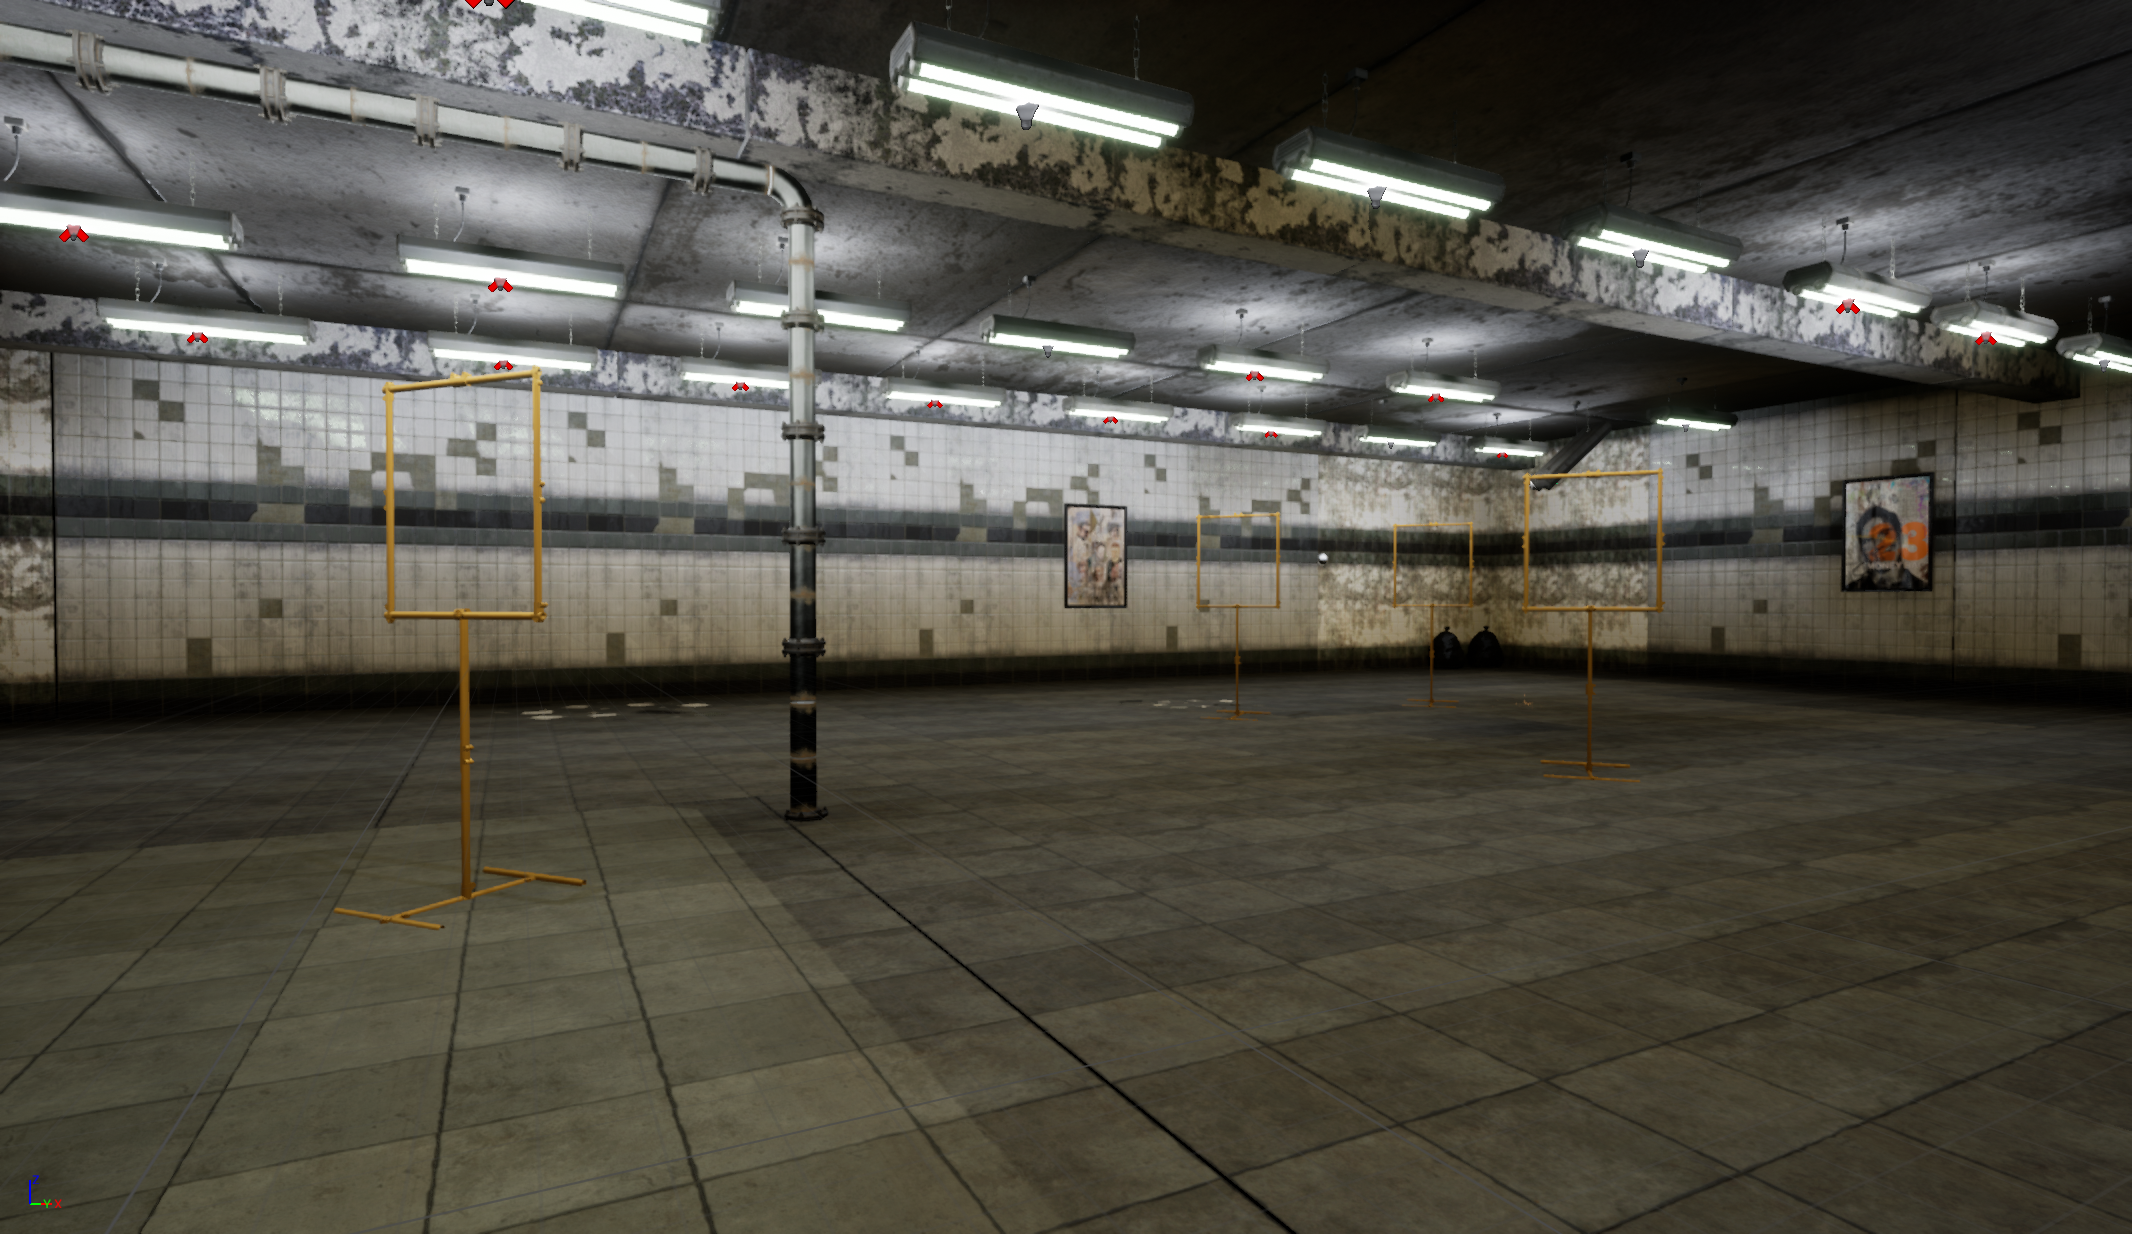
\includegraphics[width=\textwidth]{fig/basement_perspective}
	\end{minipage}
	\begin{minipage}{0.3\textwidth}
		\includegraphics[width=\textwidth]{fig/daylight_perspective}
	\end{minipage}
	\begin{minipage}{0.3\textwidth}
		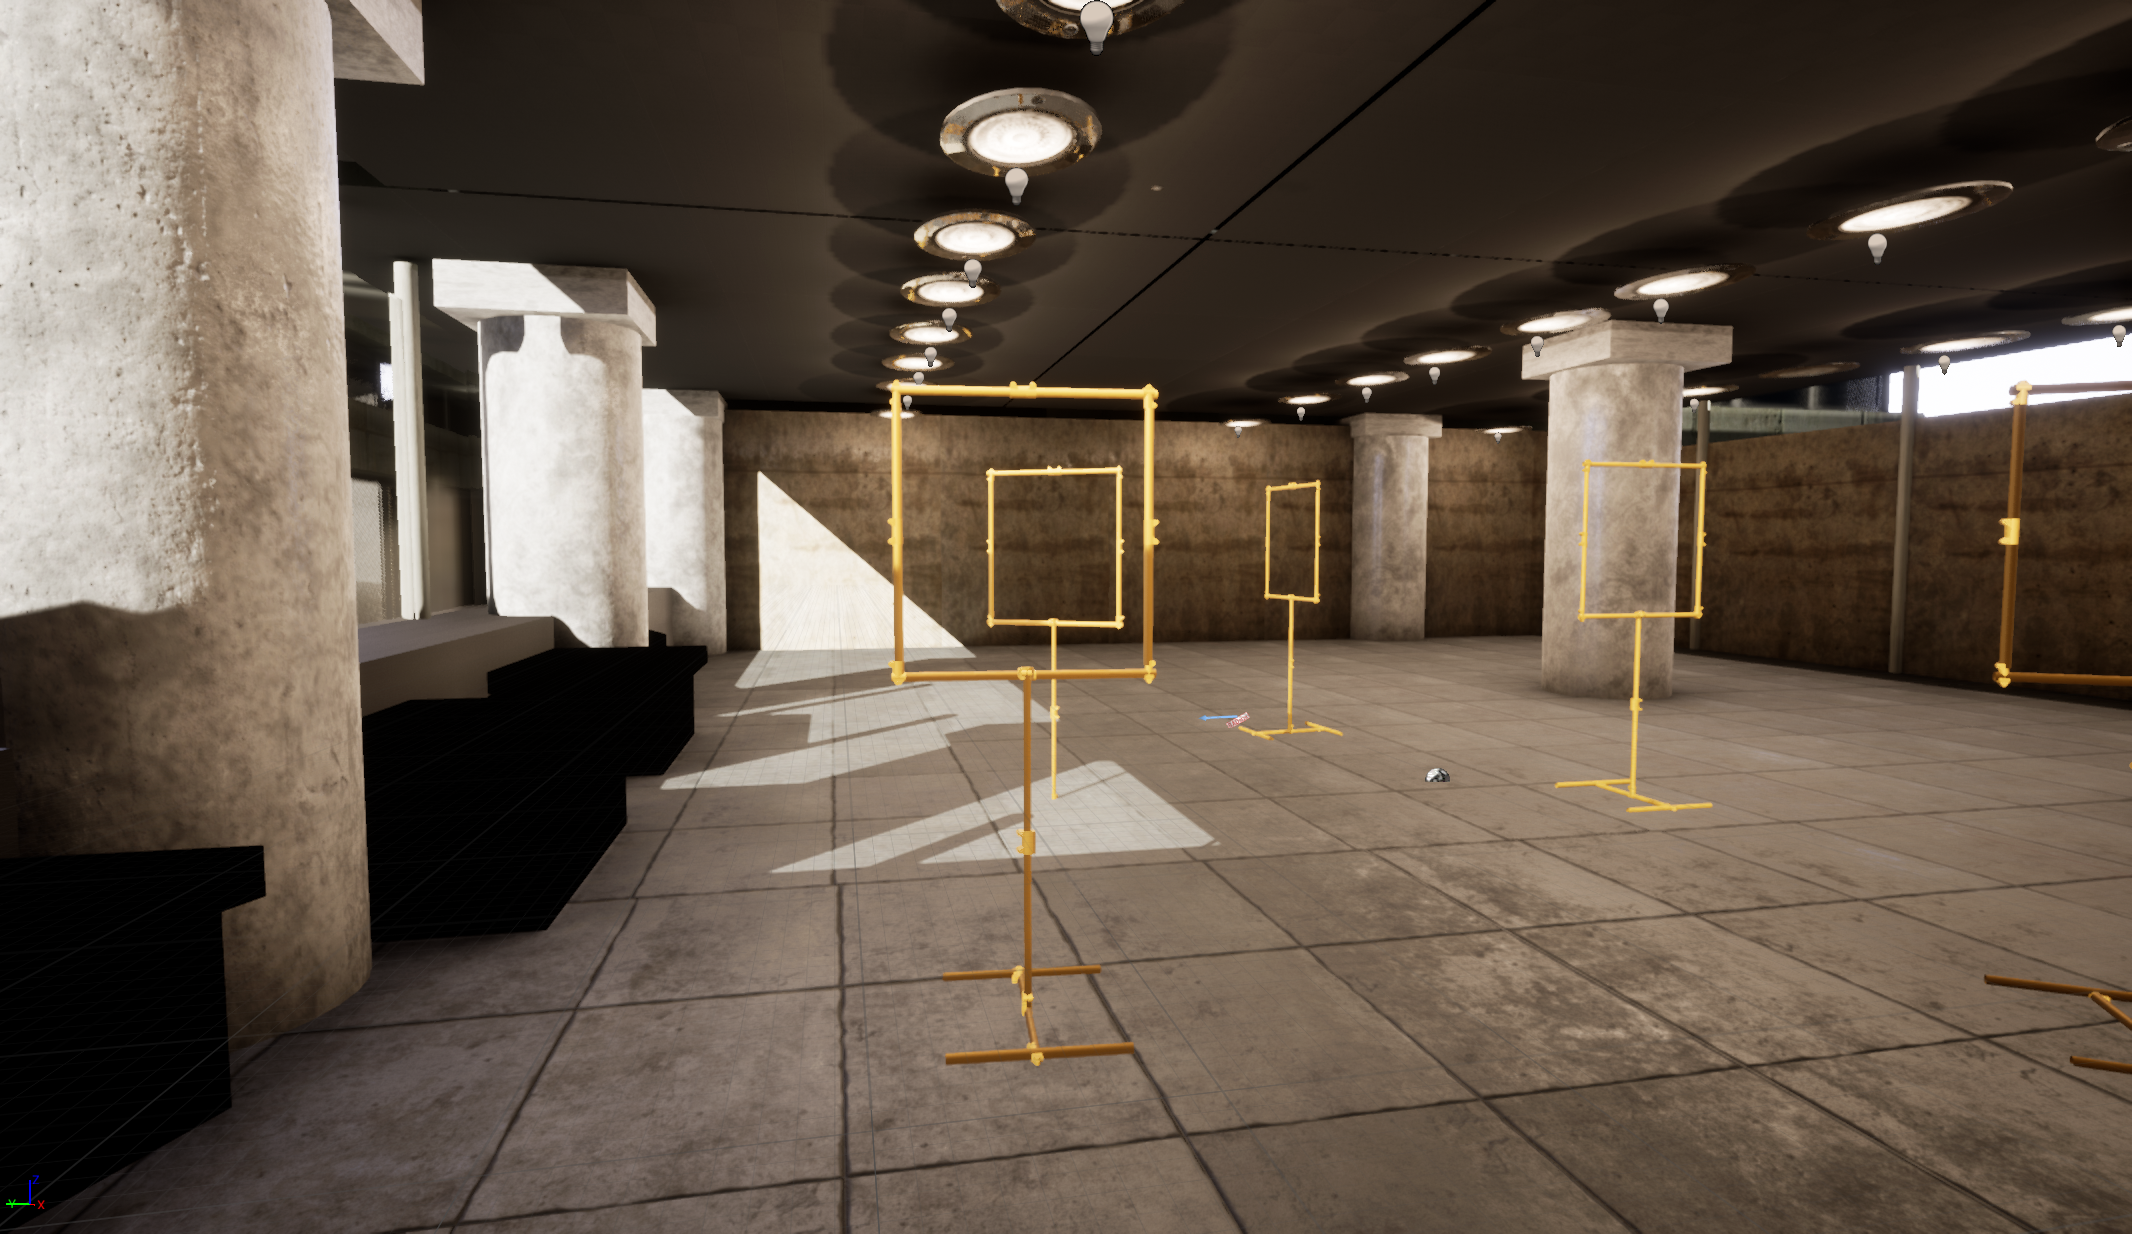
\includegraphics[width=\textwidth]{fig/iros_perspective}
	\end{minipage}
	\caption{The environments from left to right \textit{Dark}, \textit{Daylight}, \textit{IROS2018}}
	\label{fig:environments}
\end{figure}


\subsection{Post Processing}
\label{sec:postprocessing}
Another parameter that influences the image and object appearance are camera and lens conditions. An object detector should be able to cope with these effects. Hence, this work studies the influence of some effects when modeled in the training set.

Lens distortion and motion blur are chosen due to their presence in the real world data set. Furthermore, Chromatic Aberration is studied because it led to vast improvements in \cite{Carlson2018}. Variations in \ac{HSV} space are selected as it is a common image augmentation technique in current Object Detection pipelines. A visual overview can be seen in \Cref{eq:distortion}. This section describes the mathematical models behind the applied the effects.

\begin{figure}[bhtp]
	\centering
	\begin{minipage}{0.33\textwidth}
				\caption{Original Image.}
		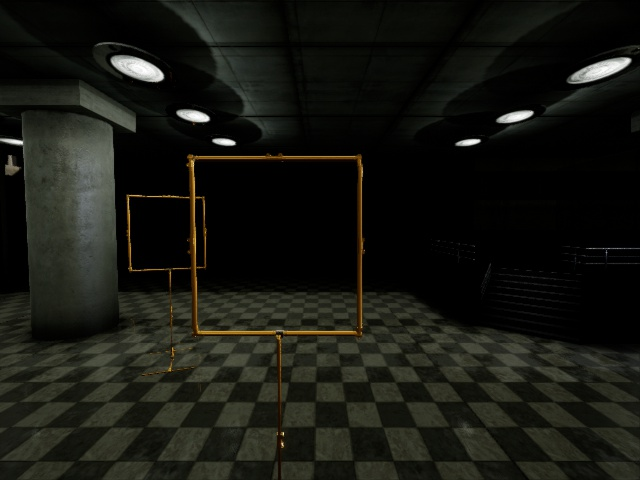
\includegraphics[width=\textwidth]{fig/gate_example}

		\label{fig:orig}
	\end{minipage}
	\begin{minipage}{0.33\textwidth}

						\caption{Chromatic Aberration. It can be seen how the red and green channel are shifted relative to each other. Thus two bars appear in the image.} 		
				
		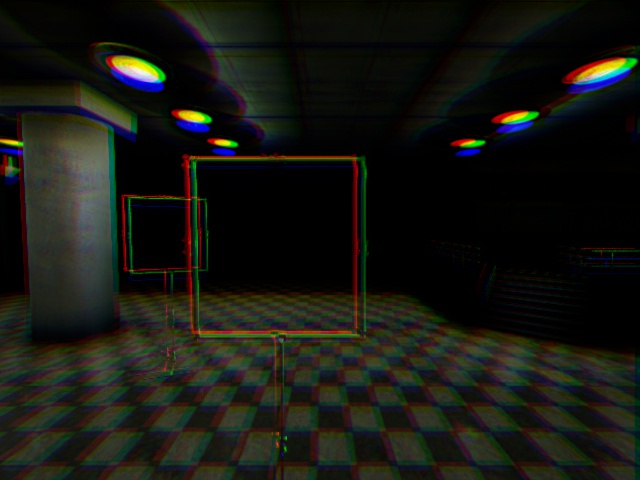
\includegraphics[width=\textwidth]{fig/gate_example_chromatic}
				\label{fig:chromatic}
	\end{minipage}
	\begin{minipage}{0.33\textwidth}
				\caption{Lens Distortion. It can be seen how the previously straight lines appear as circular shape.}
		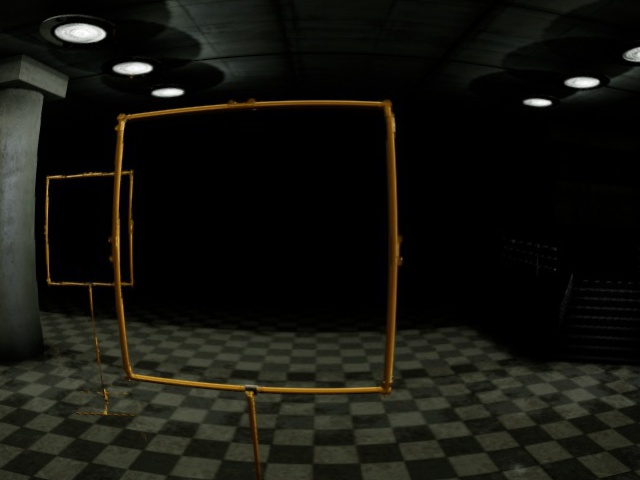
\includegraphics[width=\textwidth]{fig/gate_example_distorted}
		
		\label{fig:distortion}
	\end{minipage}
	
	\begin{minipage}{0.33\textwidth}
		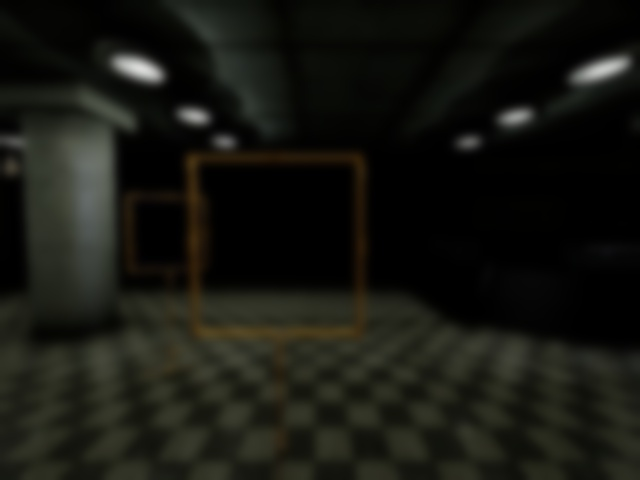
\includegraphics[width=\textwidth]{fig/gate_example_focusblur}

		\label{fig:focusblur}
	\end{minipage}
	\begin{minipage}{0.33\textwidth}
		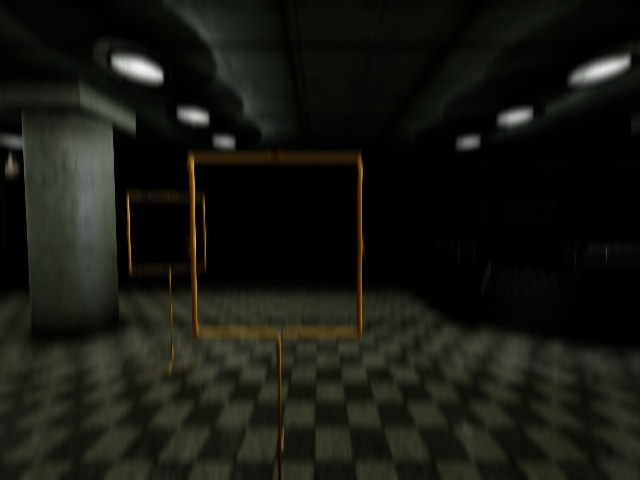
\includegraphics[width=\textwidth]{fig/gate_example_motionblur_v}
		\caption{Vertical Motion Blur.}
		\label{fig:motionblur}
	\end{minipage}
\end{figure}


\paragraph{Lens Distortion}

Lens distortion is a form of optical aberration which causes light to not fall in a single point but a region of space. For \acp{MAV} commonly used wide-angle lenses, this leads to barrel distortion and thus to straight lines appearing as curves in the image.

The effect is applied using the model for wide-angle lenses from \cite{Vass}. It models the removal of lens distortion as combination of radial and non-radial part, that is approximated with a second order Taylor expansion:

\begin{equation}
\begin{pmatrix}
p_x^u \\
p_y^u  
\end{pmatrix}=
f(p_x,p_y) =
\begin{pmatrix}
p_x (1 + \kappa_1 p_x^2 + \kappa_1 (1 + \lambda_x) p_y^2 + \kappa_2(p_x^2 + p_y^2)^2) \\
p_y (1 + \kappa_1 p_x^2 + \kappa_1 (1 + \lambda_y) p_y^2 + \kappa_2(p_x^2 + p_y^2)^2)
\end{pmatrix} 
\label{eq:distortion}
\end{equation}
Where:
\begin{itemize}
	\item $p_x^u$ and $p_y^u$ are the undistorted coordinates.
	\item $\kappa_1$ $\kappa_2$ control the radial distortion 
	\item $\lambda_x$ and $\lambda_y$ control the tangential distortion
\end{itemize}

Applying the lens distortion to an image is done by inverting \Cref{eq:distortion}. Since there is no closed form solution the Newton-approximation is used.


\paragraph{Chromatic Aberration.}

Chromatic Aberration is caused when different wavelengths of light do not end up in the same locations of the visual sensor. This leads to a shift in the colour channels of the image.

In \cite{Carlson2018} including chromatic aberration significantly improves the performance of models that are trained on fully synthesized data. Hence, we hypothesizes this will also help for our work.

Similarly to \cite{Carlson2018}, chromatic aberration is applied by scaling the locations of the green channel, as well as applying translations on all channels. Mathematically this is:

\begin{equation}
\begin{pmatrix}
p_x^c \\
p_y^c  
\end{pmatrix}= f(p_x^c,p_y^c) = \begin{pmatrix}
s^c p_x^c + t_x^c \\
s^c p_y^c + t_y^c \\
\end{pmatrix} 
\end{equation}

Where $c$ is a colour channel.

\paragraph{Blur}

Fast movement and sensor noise can lead to blurry images. This is particularly present in the domain of \ac{MAV}/Autonomous Drone Racing. Hence, we hypothesize including this effect will improve the detection in the real world. 

The effect is modelled using a Gaussian-filter. The image is convolved with a 2D-kernel build from:

\begin{equation}
k(x,y) = \frac{1}{2\sigma_x\sigma_y\pi}e^{-\frac{1}{2}({\frac{(x-\mu_x)^2}{\sigma_x^2} + \frac{(y-\mu_y)^2}{\sigma_y^2}})}
\end{equation}

Where $\sigma_x$ and $\sigma_y$ are the variance in direction x and y, used to model directional (motion) blur and $\mu_x$, $\mu_y$ are at the kernel center. 

\paragraph{Variations in \ac{HSV}}

The 3D-models and textures used in the simulator are limited and creating a large variation in environments or objects requires manual effort. An alternative method to increase the variation in colour and illumination is directly varying the colour. The \ac{HSV} colour space groups colours that are visually close to each other. Hence, for augmentation the image can be varied in this space. 
 

\section{You only look once V3 - Object Detector}

This work investigates the detection of \acp{EWFO} with \textit{YoloV3} a typical one stage detector with anchor boxes. The fundamental concept of one-stage detectors with anchor boxes is explained in \Cref{sec:related}. This section describes the detailed implementation of \textit{YoloV3} and its training goal. It further introduces the baseline network architectures of this work.

\subsection{Concept}

On a high level basis \textit{YoloV3} maps the input image to a fixed set of bounding boxes. For each box the network predicts an object probability $\hat o$ that classifies the class as object (1) or background (0). The original version of \textit{YoloV3} further distinguishes between object classes, however this work considers the single class case. There we remove this output node from the prediction. 

The anchor boxes have a predefined width $p_w$, height $p_h$ as well as a center location $c_x$,$c_y$ and are arranged in $G$ 2D-Grids with individual spatial resolution $S_n$. This allows to define different output resolutions depending on the object size. Smaller objects need a more fine grain resolution as more of them can appear close to each other. The same fine grain resolution can be too high for larger objects and thus lead to confusion of the detector during training. The bounding box dimensions $p_w$ and $p_h$ can be chosen manually or determined by k-means clustering on label width and height of the training set.

The predefined anchors only cover a subset of possible areas that can contain an object. Hence, \textit{YoloV3} also predicts how to adapt the anchor box to better fit the predicted object. These are the bounding box center $b_x,b_y$ as well as its width $b_w$ and height $b_h$. 

In total this leads to 5 predicted parameters for each bounding box and to a mapping from the input image of $I_H\times I_W\times I_D$ to $5B$ nodes that encode $B=\sum_{i=0}^{G}S^h_i\times S^w_i\times a_i$ boxes. Where $a_i$ is the number of anchor boxes in grid $i$. In a last step boxes that contain the same class prediction and have high overlap are filtered such that only the boxes with the highest confidence remain.	

\subsection{Architectures}

This mapping is implemented with a \ac{CNN}. Thereby the dimension of the network output corresponds to $S^w_*\times S^h_*\times 5a_i$.

With \textit{YoloV3} the \textit{TinyYoloV3} network was released that is 10 layer \acp{CNN} and thus a suitable baseline for this work. However, due to the small amount of layers, the receptive field of the network is only 223 pixels. Furthermore, the spatial resolution of 13x13 is still fine for objects that almost cover the whole image. Therefore the architecture is extended by an additional pooling and output layer. 

The network architecture is referred to as \textit{SmallYoloV3} and displayed in \Cref{fig:tinyyolov3_arch} and explained in detail in the following. The input image with a resolution of 416x416x3 is processed by 5 layers that stepwise decrease the spatial resolution (max pooling) while increasing the width, leading to a intermediate volume of 26x26x512. This part can be seen as a common part that extracts features for objects at all scales. The architecture is a typical example of current \acp{CNN}. In the early layers the receptive field of the filters is small. Hence, the patterns that can be represented are not very complex and only a small amount of filters is used. As the network gets deeper more complex patterns can be present and more weights are required to encode these features. Hence, the width is increased. Research has shown that fixing kernels to a size of 3x3 and stacking them in deep layers is particularly efficient \todoref{vgg}. This can also be seen in the \textit{TinyYoloV3}\todo{update picture} architecture. 

Convolving the wide volume of deeper layers such as the 26x26x512  output of layer 5 with a 3x3 kernel requires many computations. Therefore a common technique is to first compress the volume by applying a 1x1 kernel intermediately. Such \textit{bottleneck} layers can be seen in layer 6-1 and 7-2.

From layer 5 the network splits to two branches responsible for smaller and larger objects. The lower branch extracts features for larger objects leading to a final grid of 13x13. The higher branch extracts features for smaller objects leading to a grid of 26x26.

The created network serves as a baseline since it is relatively shallow and suits to the computational requirement of an \ac{MAV}. In order to study the influence of network complexity on the detection of \acp{EWFO} a second much deeper architecture is created. Its architecture is displayed in \Cref{fig:tinyyolov3_arch} and follows a similar pattern as \textit{SmallYoloV3}. However, it contains much more parameters.

\begin{figure}[hbtp]
	\centering
	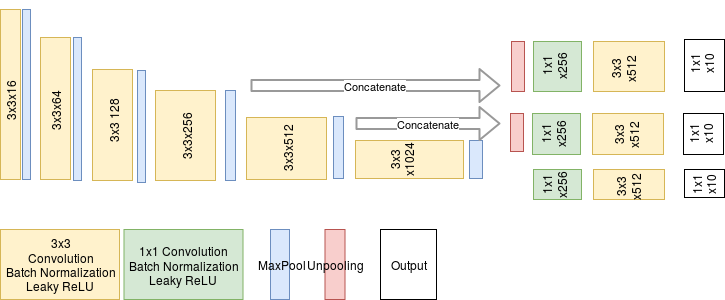
\includegraphics[width=0.8\textwidth]{fig/SmallYoloV3}
	\caption{\textit{SmallYoloV3}. In the common part the spatial resolution decreases each layer down to 26x26, while the width increases from 16 to 512. From layer 5 three branches focus on objects corresponding to different scales. }
	\label{fig:tinyyolov3_arch}
\end{figure}

\begin{figure}[hbtp]
	\centering
	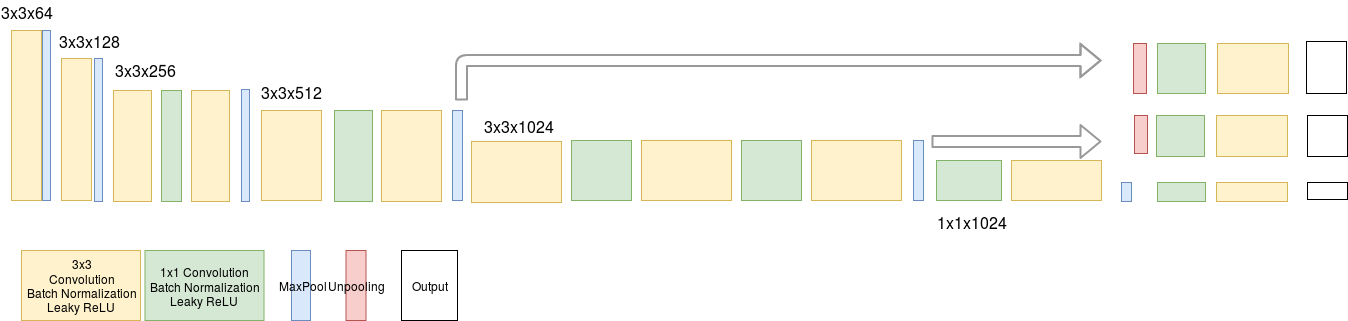
\includegraphics[width=0.8\textwidth]{fig/VGGYoloV3}
	\caption{\textit{VGGYoloV3}. A \textit{YoloV3} architecture based on \textit{VGG-19}. Similar to \textit{SmallYoloV3} the width is increased as the network gets deeper and spatial resolution decreases, while three output grids focus on different object scales. The network contains additional layers in the different stages. The bottleneck layers add flexibility without adding too much computations. }
	\label{fig:vggyolov3_arch}
\end{figure}

\subsection{Training Goal}

In order to train a \ac{CNN} to predict the desired properties a ground truth has to be defined for each output node. Subsequently the loss is formulated as derivable function and the \ac{CNN} can be trained with backpropagation.

Thereby it is desirable that a network output of zero corresponds to no filter activation and henceforth to keep all predicted bounding boxes in the default shape. Therefore, \textit{YoloV3} encodes the ground true coordinates as follows:

\begin{equation}
\label{sec:encoding}
b_x = \sigma(\hat x_{i,j,k}) + g^x_{i,j}\quad
b_y = \sigma(\hat y_{i,j,k}) + g^y_{i,j}\quad
b_w = e^{\hat w_{i,j,k}} \cdot p^w_{i,j,k}\quad
b_h = e^{\hat h_{i,j,k}} \cdot p^h_{i,j,k}
\end{equation}

where $\hat{x}$,$\hat{y}$,$\hat w_{i,j,k}$ and $\hat h_{i,j,k}$ correspond to output nodes of anchor box at grid $i$, cell $j$, anchor $k$; $g^x_{i,j,k}$, $g^y_{i,j}$ is the top left coordinate of the respective grid cell; $\sigma$ is the sigmoid-function.

The question remains to which grid cell and anchor box a label is assigned to. During training the loss is only propagated through the nodes that correspond to the "responsible" anchor box. This responsibility determined by the center location of the ground truth box and its width and height. A label is assigned to the grid in which its center falls into and within that cell to the anchor that has the highest \ac{IoU}. This can be a very strict assignment when an object has a high overlap with multiple anchor boxes. While other one stage detectors allow multiple anchors to be responsible to predict a box, \textit{YoloV3} only assigns one anchor, but ignores the predictions of an output node that has an \ac{IoU} of more than 0.5.

With true and predicted label the training goal can be formulated. The loss needs to capture the localization and the classification goal. In a typical ground truth image only a small subset of anchors is assigned responsible to predict an object. All the other anchors see only background. Hence, there is a class imbalance between the "object" class and the "background" class. Treating both losses equally would lead the model to simply assign "background" for all anchors. The weight terms $\lambda_{obj}$ and $\lambda_{noobj}$ compensate for this class imbalance. Furthermore, $\lambda_{loc}$ trades-off the localization goal and the classification goal. The abstract training loss is summarized in: 

\begin{equation}
\mathcal{L} = \lambda_{loc}\mathcal{L}_{loc} + \lambda_{obj}\mathcal{L}_{obj} + \lambda_{noobj}\mathcal{L}_{noobj} + \lambda_{class}\mathcal{L}_{class}
\end{equation}
where $\mathcal{L}_{loc}$ is the loss for bounding box dimensions, $\mathcal{L}_{obj}$ the loss where a object is present, $\mathcal{L}_{noobj}$ the loss where there is no object. The weights are kept to the default value of $\lambda_{loc} = 5$,$\lambda_{obj} = 5$ and $\lambda_{noobj} = 0.5$.

The object loss quantifies a binary classification loss. Hence, it is the difference between a predicted probability $\hat o$ and an actual class label $c$. Where $o \in \{0,1\}$ and $\hat o \in (0,1)$. In order to learn such a goal it is desirable that the weights of the network get updated significantly when the difference between truth and prediction are high. However, when prediction and truth are already close to each other, the updates to the weights should be smaller otherwise the training might miss the optimal solution. A loss function that contains the desired properties and is used by \textit{YoloV3} is the logarithmic loss which can be formulated as follows:

\begin{equation}
\mathcal{L}_{log} = -(o_{ij}\log(\hat o_{ijk}) + (1 - o_{ij})\log(1 - \hat o_{ijk}))
\end{equation}

where $\hat o_{ij}$ is an output node with sigmoid activation assigned to anchor box $i$,$j$,$k$ and $ o_{ij}$ the ground truth label assigned to that box. The logarithmic loss is calculated for each output grid $G_i$, for each grid cell $S_j$ and each anchor box $B_k$. However, only the loss of the responsible anchor boxes are summed in the total loss calculation:

\begin{equation}
\mathcal{L}_{obj} = \sum_{i=0}^{G}\sum_{j=0}^{S_i^2}\sum_{k=0}^{B_i} \mathbb{1}_{ijk}^{obj}(-(c_{ijk}\log(\hat c_{ijk}) + (1 - c_{ijk})\log(1 - \hat c_{ijk})))
\end{equation}

Thereby the  binary variable $\mathbb{1}_{ijk}^{obj}$ is 1 if an the anchor box at $i,j,k$ is assigned responsible to predict the respective object. $\mathcal{L}_{obj}$ is defined vice versa but controlled by the $\mathbb{1}_{ijk}^{noobj}$ binary variable.

For the localization loss, similar properties are desirable, although the loss should be invariant to direction. A loss that contains these properties is the squared distance between each bounding box parameter. The localization loss is summarized in:

\begin{equation}
\mathcal{L}_{loc} = \sum_{i=0}^{G} \sum_{j=0}^{S_i^2}\sum_{k=0}^{B_i} \mathbb{1}_{ijk}^{obj}[(x_{ijk}-\hat{x}_{ijk})^2 + (y_{ijk}-\hat{y}_{ijk})^2  + (w_{ijk}-\hat{w}_{ijk})^2 +(h_{ijk}-\hat{h}_{ijk})^2 ]
\end{equation}
where $x_{ijk}$,$y_{ijk}$ are the ground truth center coordinates of anchor box $i,j,k$ and $w_{ijk}$,$h_{ijk}$ the corresponding width and height. $\hat x_{ijk}$,$\hat y_{ijk}, \hat w_{ijk}$,$\hat h_{ijk}$ are the predicted bounding box coordinates. 

\subsection{Training Procedure}

With a quantified loss the training can be formalized as minimization problem: 

\begin{equation}
	\min\limits_{w}	\mathcal{L}(f(I,w),y)
\end{equation}
where $I$ is an input image, $w$ are the network weights and $y$ is the true label.

The optimization can be performed using gradient descent. However, with large amounts of data and high amount of parameters this algorithm has a slow update rate. Hence, \textit{Adam}\cite{Kingma2014}, a version of stochastic gradient descent is used. Thereby the gradient is estimated based on a subsample of the training set. While this leads to faster convergence, estimation errors can cause updates in the wrong direction. \textit{Adam} compensates for this by not only taking the mean gradient into account but also its first and second statistical moment. The three moments are weighted with $\alpha$,$\beta_1$ and $\beta_2$, where $\alpha$ is also referred to as learning rate. This work uses the parameters recommended in the initial public publication of \textit{Adam}\cite{Kingma2014}:

$$\alpha=0.001 \quad \beta_1=0.9 \quad \beta_2=0.999$$

An optimization process such as the training of a \acp{CNN} depends on the initialization of its parameters. \citeauthor{Glorot2010} \cite{Glorot2010} propose to initialize weights based on a uniform distribution centered around zero, where the borders depend on the input size of the layer. This scheme is a standard in Deep Learning frameworks and also used in this work.

\textit{YoloV3} and its training is implemented using \textit{keras} \cite{keras} with \textit{tensorflow} \cite{tensorflow} backend. 

\section{Datasets}
\label{sec:datasets}

For the objects investigated in this work no public dataset is available. Hence, two datasets are created in order to compare the performance of different detectors/architectures.

\subsection{Real-World Dataset}

A dataset has been recorded to serve as a benchmark for the developed methods. The dataset consists of 300 images recorded with the JeVois camera during flight and while remaining on ground. The samples stem from three different rooms with varying light conditions. The rooms are referred to as \textit{Basement}, \textit{Cyberzoo} and \textit{Hallway}. Example images for each room can be seen in \Cref{fig:example_real_set}.
\begin{figure}
	\centering
	\begin{minipage}{0.3\textwidth}
		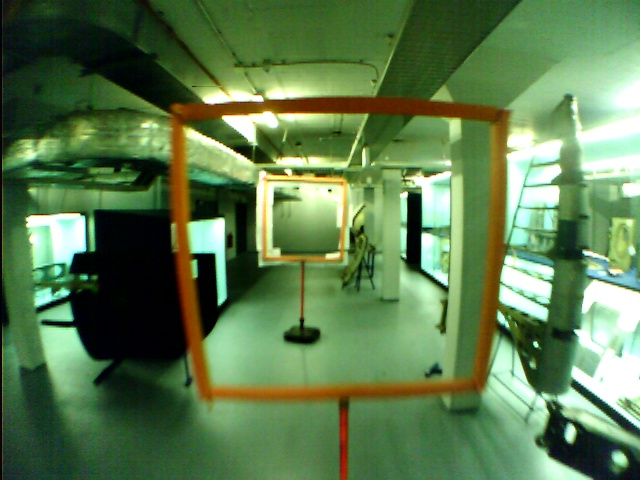
\includegraphics[width=\textwidth]{fig/basement}
	\end{minipage}\hfill
	\begin{minipage}{0.3\textwidth}
		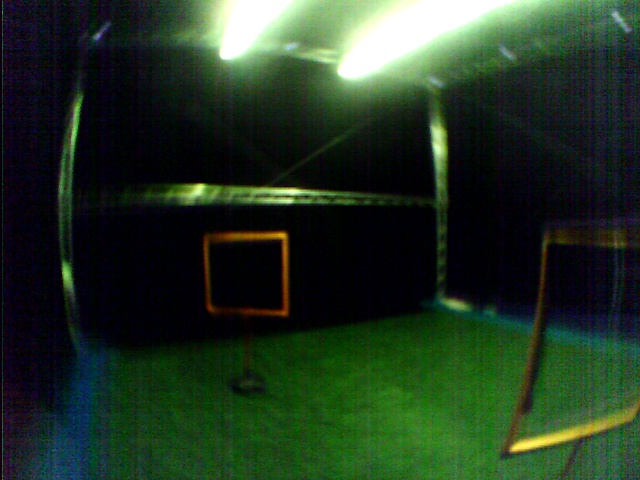
\includegraphics[width=\textwidth]{fig/cyberzoo}
	\end{minipage}\hfill
	\begin{minipage}{0.3\textwidth}
		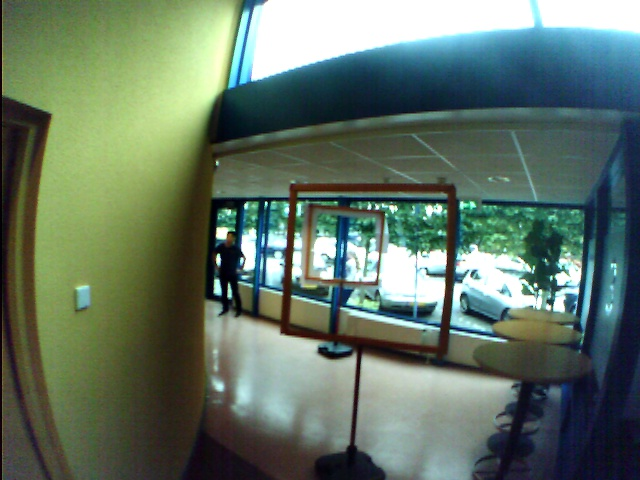
\includegraphics[width=\textwidth]{fig/hallway}
	\end{minipage}
	\caption{Examples of the three test domains. From left to right: \textit{Basement}, \textit{Cyberzoo} and \textit{Hallway}}
	\label{fig:example_real_set}
\end{figure}

All environments are indoor scenes which are a typical examples for GPS-denied areas, where vision based state estimation is required. The scenes contain two gates that are arranged in varying order. Hence up to two objects are visible and can overlap which means the gate farer away can be seen through the closer gate. Each of the rooms has different environmental conditions:
\begin{enumerate}
	\item \textit{Basement} is a bright environment illuminated by artificial light sources. The corridor in which the objects of interest are placed are narrow while also objects and persons are visible on the samples. The dataset contains 163 samples with 312 objects in total.
	\item \textit{Cyberzoo} is taken from a test environment for \ac{MAV} flights.  It is surrounded by black curtains such that an even illumination and dark background is created. Only in a small subset of images distractors like other objects or persons are visible. In total 88 samples stem from this room while 71 objects are present.
	\item \textit{Hallway} is a bright environment illuminated by a combination of artificial light sources as well as daylight that shines through the windows. The samples are taken with the windows as background. This leads to a very bright background such that the thin structure of the objects are hardly visible. The dataset contains 49 samples with a total of 86 objects.
\end{enumerate}


\subsection{Test Set in Simulation}

The data that can be created with the data generation tool is limited by the graphical engine, the used textures and the created environments. It is possible that this reality gap limits the performance of the detection on real data. Hence, only measuring the performance on the real world dataset would limit the insights gained from the experiments. That is why a synthetic test set is created by simulating a flight through the \textit{IROS}-environment. This also allows to evaluate the performance of the detection network on race courts with more than two gates and at view angles that are not present in the real world dataset.  

The arrangement of racing gates is based on the race court of the Autonomous Drone Race at \ac{IROS} 2018. This test set contains 550 images with a total of 1361\todo{recount with filtered} objects.



